\chapter{An Appendix}

\begin{figure} [H]
	\begin{minipage}{\textwidth}
		\centering
		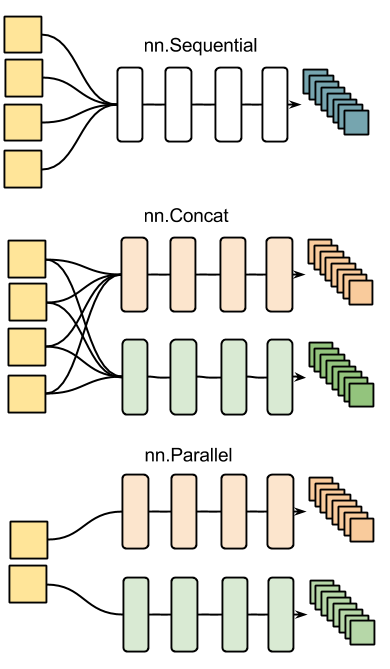
\includegraphics[width=0.5\linewidth]{figure/nncontainer}
		\caption[A parsed sentence in SST]{A parsed sentence in SST \footnote{ \url{https://github.com/soumith/cvpr2015/blob/master/Deep\%20Learning\%20with\%20Torch.ipynb}}}
		\label{fig:nncontainer}
	\end{minipage}
\end{figure}

\begin{lstlisting}[caption={MLP using nngraph},label={lst:torchtrain}, language={[5.1]Lua}]
require 'nn'
require 'optim'

model = nn.Sequential()
model:add(nn.Linear(1,1))

criterion = nn.MSECriterion()

x = torch.Tensor{{1,2,3,4,5,6,7,8,9,10}}
x = x:t()
y = torch.Tensor{{3,5,7,9,11,13,15,17,19,21}}
y = y:t()

params, gradParams = model:getParameters()

function feval(params)
	gradParams:zero()
	local outputs = model:forward(x)
	local loss = criterion:forward(outputs,y)
	local dloss_doutput = criterion:backward(outputs,y)
	model:backward(x, dloss_doutput)
	return loss, gradParams
end

local optimState = {
	learningRate = 0.01
}

for epoch = 1, 100 do
	optim.sgd(feval,params, optimState)
end

test = torch.Tensor{{1,3,5,7,9,11,100}}
test = test:t()

print (model:forward(test))
\end{lstlisting}



\begin{lstlisting}[caption={Theano MLP},label={lst:theanomlp}, language={python}]
	import numpy as np
	import theano
	import theano.tensor as T
	import theano.tensor.nnet as nnet

	class MLP:
	    def __init__(self):
	        x = T.dvector()
	        y = T.dscalar()
	        t1 = np.array(np.random.rand(3, 3), dtype=theano.config.floatX)
	        theta1 = theano.shared(t1)  # 3x3 weight matrix
	        t2 = np.array(np.random.rand(4, 1), dtype=theano.config.floatX)
	        hid1 = MLP.sigmoid_layer(x, theta1)  # hidden layer
	        theta2 = theano.shared(t2)  # 4x1 weight matrix
	        output_layer = T.sum(MLP.sigmoid_layer(hid1, theta2))
	        fc = (output_layer - y)**2
	        self.cost = theano.function(inputs=[x,y], outputs = fc,updates=[
	            (theta1, Xor.grad_desc(fc, theta1)),
	            (theta2, Xor.grad_desc(fc, theta2))
	        ])
	        self.run_forward = theano.function(inputs=[x],outputs=output_layer)

	    @staticmethod
	    def sigmoid_layer(x, w):
	        b = np.array([1], dtype=theano.config.floatX)
	        new_x = T.concatenate([x,b])
	        m = T.dot(w.T, new_x)
	        h = nnet.sigmoid(m)
	        return h


	    @staticmethod
	    def grad_desc(cost, theta):
	        alpha = 0.1
	        return theta - (alpha* T.grad(cost, wrt=theta))

	    def forward(self, x):
	        output = self.run_forward(x)
	        return output


	    def train(self, train_x, train_y, n_epoch):
	        cur_cost = 0
	        for epoch in range(n_epoch):
	            for i in range(len(train_x)):
	                cur_cost = self.cost(train_x[i],train_y[i])
	            if epoch % 1000 == 0:
	                print(cur_cost)
	        print ('train complete')
\end{lstlisting}
